% 16:9 aspect ratio so it will fill a TV screen
\documentclass[aspectratio=169]{beamer}

\usepackage{hacksoc}
\usepackage{vwcol}

% use pausefn command so you can generate slides with and without pauses
%\newcommand{\pausefn}{\pause}
\newcommand{\pausefn}{}

\title{HTML forms to REST}
\subtitle{HTTP's Newton to Einstein}
\author{Peter Taylor}
\date{\today}

\begin{document}
{
\usebackgroundtemplate{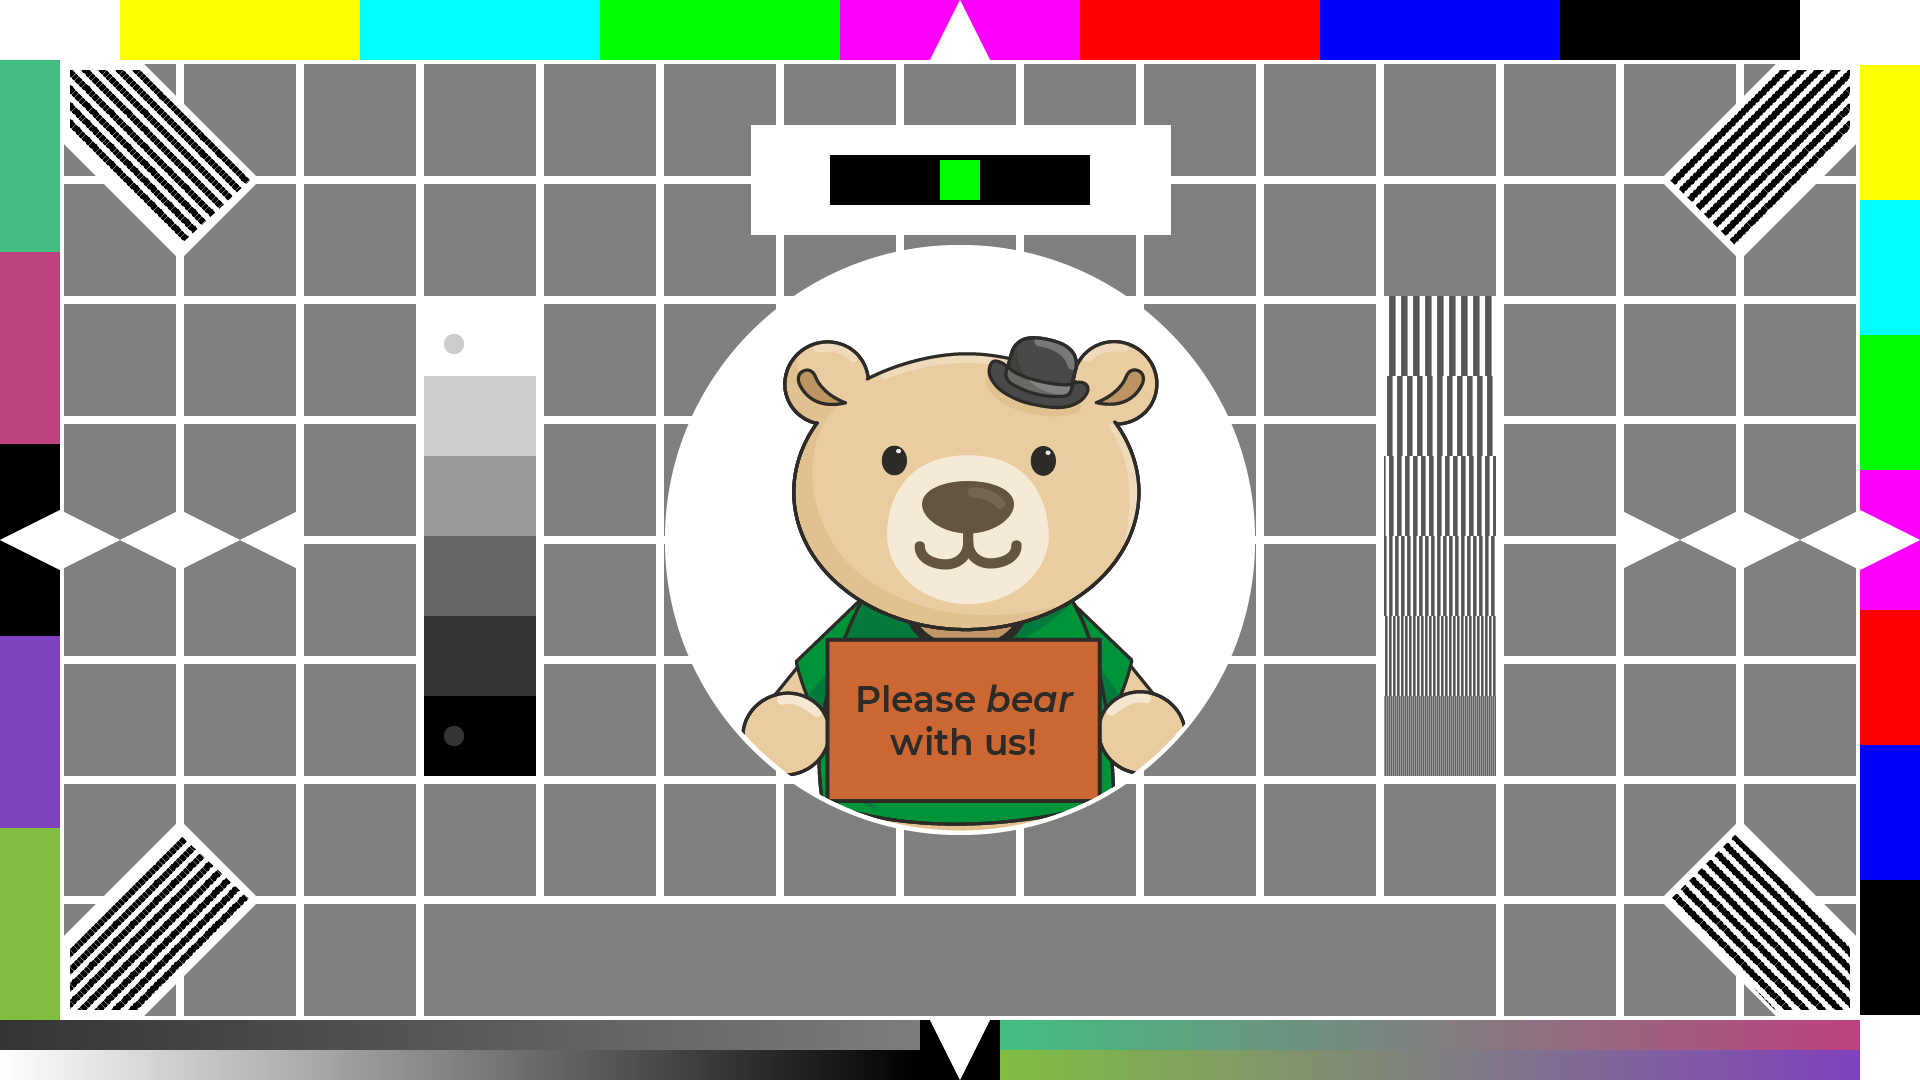
\includegraphics[width=\paperwidth]{images/HackSoc_Test_Card}}
\begin{frame}[plain]
\end{frame}
}

% Title slide
\maketitleslide

% Section Names have their own slides generated, make sure they are out of a frame
% environment. If you want it numbered, include it in the name of the section
\section{Part I: HTML Forms}

\begin{frame}
  \frametitle{POST HTML Forms}
  \begin{columns}
    \begin{column}{0.6\textwidth}
      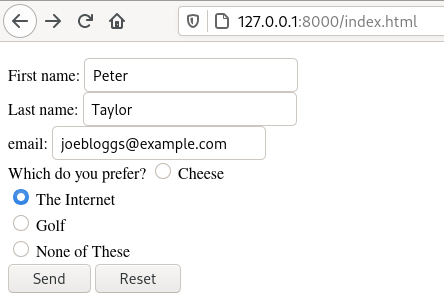
\includegraphics[width=8cm]{form.png}\\    
    \end{column}
  
    \begin{column}{0.35\textwidth}
      \begin{itemize}
        \item HTML forms provide a method for the user to send data to the server
        \item This is a post form with a variety of data inputs
        \item This data is then sent in an HTTP POST request back to the server
      \end{itemize}
    \end{column}
  \end{columns}
\end{frame}

\begin{frame}
  \frametitle{Dissecting an HTTP Request}

\texttt{POST / HTTP/1.1} \textbf{- The HTTP Method} \pause\\
{\tiny
\texttt{Host: 127.0.0.1:8000}\\
\texttt{User-Agent: Mozilla/5.0 (X11; Linux x86\_64; rv:80.0) Gecko/20100101}\\\hspace{2em} \texttt{Firefox/80.0}\\
}
\texttt{Accept: text/html,application/xhtml+xml,application/xml;}\\\hspace{2em}\texttt{q=0.9,image/webp,*/*;q=0.8}\\
{\tiny
\texttt{Accept-Language: en-US,en;q=0.5}\\
\texttt{Accept-Encoding: gzip, deflate}\pause\\
}
\texttt{Content-Type: application/x-www-form-urlencoded} \textbf{- The Format of the data}\pause\\
\texttt{Content-Length: 77} \textbf{- The Length of what we're sending}\pause\\
{\tiny
\texttt{Origin: http://127.0.0.1:8000} \\
\texttt{Referer: http://127.0.0.1:8000/index.html}\\
\texttt{Upgrade-Insecure-Requests: 1}\\
}
\texttt{ }\\
\texttt{firstname=Peter\&lastname=Taylor\&email=joebloggs\%40example.com}\\
\hspace{2em}\texttt{\&favourite=internet}\\
  
\end{frame}

\begin{frame}
  \frametitle{Sending data over HTTP}
  \begin{itemize}
    \item The \texttt{Content-Type:} line specifies the media \footnote{Formerly MIME (Multipurpose Internet Mail Extensions)} type of the data you're sending (so the server knows what how to handle)
    \item We can send/receive data in a different format that supports things like arrays
    \begin{itemize}
      \item XML\footnote{Haha no}
      \item JSON - small, widely handled and 
    \end{itemize}
  \end{itemize}
  These fix the issues with \texttt{urlencoded} being difficult to serialise and not having nice structuring (especially over having to extract data from an HTML web page)
\end{frame}

\section{Live Demo 1\footnote{What could possibly go wrong?} - AUR Search}

\begin{frame}
  \frametitle{Looking at APIs}
  \framesubtitle{Prerequisite tools}
  \textbf{Insomnia REST Debugger}\\
  \texttt{https://insomnia.rest/} Installers for Windows, brew, snap and AUR are available
  \\If you really want, you can use \texttt{curl} or another tool like postman

\end{frame}

\end{document}
